% Created by tikzDevice version 0.12.3.1 on 2021-10-17 10:40:53
% !TEX encoding = UTF-8 Unicode
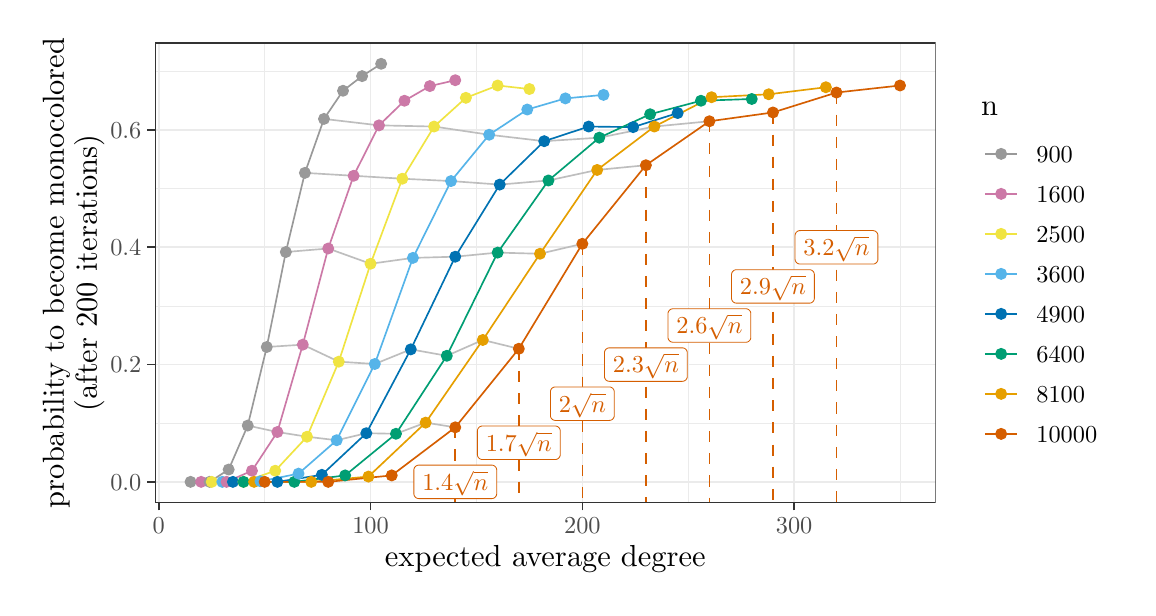
\begin{tikzpicture}[x=1pt,y=1pt]
\definecolor{fillColor}{RGB}{255,255,255}
\path[use as bounding box,fill=fillColor,fill opacity=0.00] (0,0) rectangle (397.48,202.36);
\begin{scope}
\path[clip] (  0.00,  0.00) rectangle (397.48,202.36);
\definecolor{drawColor}{RGB}{255,255,255}
\definecolor{fillColor}{RGB}{255,255,255}

\path[draw=drawColor,line width= 0.6pt,line join=round,line cap=round,fill=fillColor] (  0.00,  0.00) rectangle (397.48,202.36);
\end{scope}
\begin{scope}
\path[clip] ( 46.04, 30.69) rectangle (328.04,196.86);
\definecolor{fillColor}{RGB}{255,255,255}

\path[fill=fillColor] ( 46.04, 30.69) rectangle (328.04,196.86);
\definecolor{drawColor}{gray}{0.92}

\path[draw=drawColor,line width= 0.3pt,line join=round] ( 46.04, 59.43) --
	(328.04, 59.43);

\path[draw=drawColor,line width= 0.3pt,line join=round] ( 46.04,101.80) --
	(328.04,101.80);

\path[draw=drawColor,line width= 0.3pt,line join=round] ( 46.04,144.17) --
	(328.04,144.17);

\path[draw=drawColor,line width= 0.3pt,line join=round] ( 46.04,186.55) --
	(328.04,186.55);

\path[draw=drawColor,line width= 0.3pt,line join=round] ( 85.64, 30.69) --
	( 85.64,196.86);

\path[draw=drawColor,line width= 0.3pt,line join=round] (162.17, 30.69) --
	(162.17,196.86);

\path[draw=drawColor,line width= 0.3pt,line join=round] (238.69, 30.69) --
	(238.69,196.86);

\path[draw=drawColor,line width= 0.3pt,line join=round] (315.22, 30.69) --
	(315.22,196.86);

\path[draw=drawColor,line width= 0.6pt,line join=round] ( 46.04, 38.24) --
	(328.04, 38.24);

\path[draw=drawColor,line width= 0.6pt,line join=round] ( 46.04, 80.61) --
	(328.04, 80.61);

\path[draw=drawColor,line width= 0.6pt,line join=round] ( 46.04,122.99) --
	(328.04,122.99);

\path[draw=drawColor,line width= 0.6pt,line join=round] ( 46.04,165.36) --
	(328.04,165.36);

\path[draw=drawColor,line width= 0.6pt,line join=round] ( 47.38, 30.69) --
	( 47.38,196.86);

\path[draw=drawColor,line width= 0.6pt,line join=round] (123.90, 30.69) --
	(123.90,196.86);

\path[draw=drawColor,line width= 0.6pt,line join=round] (200.43, 30.69) --
	(200.43,196.86);

\path[draw=drawColor,line width= 0.6pt,line join=round] (276.95, 30.69) --
	(276.95,196.86);
\definecolor{drawColor}{RGB}{190,190,190}

\path[draw=drawColor,line width= 0.6pt,line join=round] ( 79.52, 58.58) --
	( 90.23, 56.25) --
	(100.94, 54.55) --
	(111.66, 53.28) --
	(122.37, 55.82) --
	(133.08, 55.61) --
	(143.80, 59.64) --
	(154.51, 57.94);

\path[draw=drawColor,line width= 0.6pt,line join=round] ( 86.40, 86.97) --
	( 99.41, 87.82) --
	(112.42, 81.67) --
	(125.43, 80.83) --
	(138.44, 86.12) --
	(151.45, 83.79) --
	(164.46, 89.51) --
	(177.47, 86.33);

\path[draw=drawColor,line width= 0.6pt,line join=round] ( 93.29,121.29) --
	(108.60,122.56) --
	(123.90,117.05) --
	(139.21,119.17) --
	(154.51,119.60) --
	(169.82,121.08) --
	(185.12,120.66) --
	(200.43,124.26);

\path[draw=drawColor,line width= 0.6pt,line join=round] (100.18,149.89) --
	(117.78,148.84) --
	(135.38,147.78) --
	(152.98,146.93) --
	(170.58,145.66) --
	(188.18,147.14) --
	(205.79,150.95) --
	(223.39,152.65);

\path[draw=drawColor,line width= 0.6pt,line join=round] (107.07,169.39) --
	(126.96,167.06) --
	(146.86,166.63) --
	(166.76,163.67) --
	(186.65,161.34) --
	(206.55,162.61) --
	(226.45,166.63) --
	(246.34,168.54);
\definecolor{drawColor}{gray}{0.60}

\path[draw=drawColor,line width= 0.6pt,line join=round] ( 58.85, 38.24) --
	( 65.74, 38.24) --
	( 72.63, 42.69) --
	( 79.52, 58.58) --
	( 86.40, 86.97) --
	( 93.29,121.29) --
	(100.18,149.89) --
	(107.07,169.39) --
	(113.95,179.56) --
	(120.84,184.85) --
	(127.73,189.30);
\definecolor{drawColor}{RGB}{204,121,167}

\path[draw=drawColor,line width= 0.6pt,line join=round] ( 62.68, 38.24) --
	( 71.86, 38.24) --
	( 81.05, 42.26) --
	( 90.23, 56.25) --
	( 99.41, 87.82) --
	(108.60,122.56) --
	(117.78,148.84) --
	(126.96,167.06) --
	(136.15,175.95) --
	(145.33,181.25) --
	(154.51,183.37);
\definecolor{drawColor}{RGB}{240,228,66}

\path[draw=drawColor,line width= 0.6pt,line join=round] ( 66.51, 38.24) --
	( 77.99, 38.24) --
	( 89.46, 42.26) --
	(100.94, 54.55) --
	(112.42, 81.67) --
	(123.90,117.05) --
	(135.38,147.78) --
	(146.86,166.63) --
	(158.34,177.01) --
	(169.82,181.46) --
	(181.30,180.19);
\definecolor{drawColor}{RGB}{86,180,233}

\path[draw=drawColor,line width= 0.6pt,line join=round] ( 70.33, 38.24) --
	( 84.11, 38.45) --
	( 97.88, 41.21) --
	(111.66, 53.28) --
	(125.43, 80.83) --
	(139.21,119.17) --
	(152.98,146.93) --
	(166.76,163.67) --
	(180.53,172.78) --
	(194.31,176.80) --
	(208.08,178.07);
\definecolor{drawColor}{RGB}{0,114,178}

\path[draw=drawColor,line width= 0.6pt,line join=round] ( 74.16, 38.24) --
	( 90.23, 38.24) --
	(106.30, 40.78) --
	(122.37, 55.82) --
	(138.44, 86.12) --
	(154.51,119.60) --
	(170.58,145.66) --
	(186.65,161.34) --
	(202.72,166.63) --
	(218.79,166.42) --
	(234.87,171.51);
\definecolor{drawColor}{RGB}{0,158,115}

\path[draw=drawColor,line width= 0.6pt,line join=round] ( 77.99, 38.24) --
	( 96.35, 38.24) --
	(114.72, 40.57) --
	(133.08, 55.61) --
	(151.45, 83.79) --
	(169.82,121.08) --
	(188.18,147.14) --
	(206.55,162.61) --
	(224.92,171.08) --
	(243.28,175.95) --
	(261.65,176.59);
\definecolor{drawColor}{RGB}{230,159,0}

\path[draw=drawColor,line width= 0.6pt,line join=round] ( 81.81, 38.24) --
	(102.47, 38.24) --
	(123.14, 40.15) --
	(143.80, 59.64) --
	(164.46, 89.51) --
	(185.12,120.66) --
	(205.79,150.95) --
	(226.45,166.63) --
	(247.11,177.23) --
	(267.77,178.29) --
	(288.43,180.83);
\definecolor{drawColor}{RGB}{213,94,0}

\path[draw=drawColor,line width= 0.6pt,line join=round] ( 85.64, 38.24) --
	(108.60, 38.24) --
	(131.55, 40.57) --
	(154.51, 57.94) --
	(177.47, 86.33) --
	(200.43,124.26) --
	(223.39,152.65) --
	(246.34,168.54) --
	(269.30,171.72) --
	(292.26,178.92) --
	(315.22,181.46);
\definecolor{drawColor}{gray}{0.60}
\definecolor{fillColor}{gray}{0.60}

\path[draw=drawColor,line width= 0.4pt,line join=round,line cap=round,fill=fillColor] ( 58.85, 38.24) circle (  1.96);
\definecolor{drawColor}{RGB}{204,121,167}
\definecolor{fillColor}{RGB}{204,121,167}

\path[draw=drawColor,line width= 0.4pt,line join=round,line cap=round,fill=fillColor] ( 62.68, 38.24) circle (  1.96);
\definecolor{drawColor}{gray}{0.60}
\definecolor{fillColor}{gray}{0.60}

\path[draw=drawColor,line width= 0.4pt,line join=round,line cap=round,fill=fillColor] ( 65.74, 38.24) circle (  1.96);
\definecolor{drawColor}{RGB}{240,228,66}
\definecolor{fillColor}{RGB}{240,228,66}

\path[draw=drawColor,line width= 0.4pt,line join=round,line cap=round,fill=fillColor] ( 66.51, 38.24) circle (  1.96);
\definecolor{drawColor}{RGB}{86,180,233}
\definecolor{fillColor}{RGB}{86,180,233}

\path[draw=drawColor,line width= 0.4pt,line join=round,line cap=round,fill=fillColor] ( 70.33, 38.24) circle (  1.96);
\definecolor{drawColor}{RGB}{204,121,167}
\definecolor{fillColor}{RGB}{204,121,167}

\path[draw=drawColor,line width= 0.4pt,line join=round,line cap=round,fill=fillColor] ( 71.86, 38.24) circle (  1.96);
\definecolor{drawColor}{gray}{0.60}
\definecolor{fillColor}{gray}{0.60}

\path[draw=drawColor,line width= 0.4pt,line join=round,line cap=round,fill=fillColor] ( 72.63, 42.69) circle (  1.96);
\definecolor{drawColor}{RGB}{0,114,178}
\definecolor{fillColor}{RGB}{0,114,178}

\path[draw=drawColor,line width= 0.4pt,line join=round,line cap=round,fill=fillColor] ( 74.16, 38.24) circle (  1.96);
\definecolor{drawColor}{RGB}{240,228,66}
\definecolor{fillColor}{RGB}{240,228,66}

\path[draw=drawColor,line width= 0.4pt,line join=round,line cap=round,fill=fillColor] ( 77.99, 38.24) circle (  1.96);
\definecolor{drawColor}{RGB}{0,158,115}
\definecolor{fillColor}{RGB}{0,158,115}

\path[draw=drawColor,line width= 0.4pt,line join=round,line cap=round,fill=fillColor] ( 77.99, 38.24) circle (  1.96);
\definecolor{drawColor}{gray}{0.60}
\definecolor{fillColor}{gray}{0.60}

\path[draw=drawColor,line width= 0.4pt,line join=round,line cap=round,fill=fillColor] ( 79.52, 58.58) circle (  1.96);
\definecolor{drawColor}{RGB}{204,121,167}
\definecolor{fillColor}{RGB}{204,121,167}

\path[draw=drawColor,line width= 0.4pt,line join=round,line cap=round,fill=fillColor] ( 81.05, 42.26) circle (  1.96);
\definecolor{drawColor}{RGB}{230,159,0}
\definecolor{fillColor}{RGB}{230,159,0}

\path[draw=drawColor,line width= 0.4pt,line join=round,line cap=round,fill=fillColor] ( 81.81, 38.24) circle (  1.96);
\definecolor{drawColor}{RGB}{86,180,233}
\definecolor{fillColor}{RGB}{86,180,233}

\path[draw=drawColor,line width= 0.4pt,line join=round,line cap=round,fill=fillColor] ( 84.11, 38.45) circle (  1.96);
\definecolor{drawColor}{RGB}{213,94,0}
\definecolor{fillColor}{RGB}{213,94,0}

\path[draw=drawColor,line width= 0.4pt,line join=round,line cap=round,fill=fillColor] ( 85.64, 38.24) circle (  1.96);
\definecolor{drawColor}{gray}{0.60}
\definecolor{fillColor}{gray}{0.60}

\path[draw=drawColor,line width= 0.4pt,line join=round,line cap=round,fill=fillColor] ( 86.40, 86.97) circle (  1.96);
\definecolor{drawColor}{RGB}{240,228,66}
\definecolor{fillColor}{RGB}{240,228,66}

\path[draw=drawColor,line width= 0.4pt,line join=round,line cap=round,fill=fillColor] ( 89.46, 42.26) circle (  1.96);
\definecolor{drawColor}{RGB}{204,121,167}
\definecolor{fillColor}{RGB}{204,121,167}

\path[draw=drawColor,line width= 0.4pt,line join=round,line cap=round,fill=fillColor] ( 90.23, 56.25) circle (  1.96);
\definecolor{drawColor}{RGB}{0,114,178}
\definecolor{fillColor}{RGB}{0,114,178}

\path[draw=drawColor,line width= 0.4pt,line join=round,line cap=round,fill=fillColor] ( 90.23, 38.24) circle (  1.96);
\definecolor{drawColor}{gray}{0.60}
\definecolor{fillColor}{gray}{0.60}

\path[draw=drawColor,line width= 0.4pt,line join=round,line cap=round,fill=fillColor] ( 93.29,121.29) circle (  1.96);
\definecolor{drawColor}{RGB}{0,158,115}
\definecolor{fillColor}{RGB}{0,158,115}

\path[draw=drawColor,line width= 0.4pt,line join=round,line cap=round,fill=fillColor] ( 96.35, 38.24) circle (  1.96);
\definecolor{drawColor}{RGB}{86,180,233}
\definecolor{fillColor}{RGB}{86,180,233}

\path[draw=drawColor,line width= 0.4pt,line join=round,line cap=round,fill=fillColor] ( 97.88, 41.21) circle (  1.96);
\definecolor{drawColor}{RGB}{204,121,167}
\definecolor{fillColor}{RGB}{204,121,167}

\path[draw=drawColor,line width= 0.4pt,line join=round,line cap=round,fill=fillColor] ( 99.41, 87.82) circle (  1.96);
\definecolor{drawColor}{gray}{0.60}
\definecolor{fillColor}{gray}{0.60}

\path[draw=drawColor,line width= 0.4pt,line join=round,line cap=round,fill=fillColor] (100.18,149.89) circle (  1.96);
\definecolor{drawColor}{RGB}{240,228,66}
\definecolor{fillColor}{RGB}{240,228,66}

\path[draw=drawColor,line width= 0.4pt,line join=round,line cap=round,fill=fillColor] (100.94, 54.55) circle (  1.96);
\definecolor{drawColor}{RGB}{230,159,0}
\definecolor{fillColor}{RGB}{230,159,0}

\path[draw=drawColor,line width= 0.4pt,line join=round,line cap=round,fill=fillColor] (102.47, 38.24) circle (  1.96);
\definecolor{drawColor}{RGB}{0,114,178}
\definecolor{fillColor}{RGB}{0,114,178}

\path[draw=drawColor,line width= 0.4pt,line join=round,line cap=round,fill=fillColor] (106.30, 40.78) circle (  1.96);
\definecolor{drawColor}{gray}{0.60}
\definecolor{fillColor}{gray}{0.60}

\path[draw=drawColor,line width= 0.4pt,line join=round,line cap=round,fill=fillColor] (107.07,169.39) circle (  1.96);
\definecolor{drawColor}{RGB}{204,121,167}
\definecolor{fillColor}{RGB}{204,121,167}

\path[draw=drawColor,line width= 0.4pt,line join=round,line cap=round,fill=fillColor] (108.60,122.56) circle (  1.96);
\definecolor{drawColor}{RGB}{213,94,0}
\definecolor{fillColor}{RGB}{213,94,0}

\path[draw=drawColor,line width= 0.4pt,line join=round,line cap=round,fill=fillColor] (108.60, 38.24) circle (  1.96);
\definecolor{drawColor}{RGB}{86,180,233}
\definecolor{fillColor}{RGB}{86,180,233}

\path[draw=drawColor,line width= 0.4pt,line join=round,line cap=round,fill=fillColor] (111.66, 53.28) circle (  1.96);
\definecolor{drawColor}{RGB}{240,228,66}
\definecolor{fillColor}{RGB}{240,228,66}

\path[draw=drawColor,line width= 0.4pt,line join=round,line cap=round,fill=fillColor] (112.42, 81.67) circle (  1.96);
\definecolor{drawColor}{gray}{0.60}
\definecolor{fillColor}{gray}{0.60}

\path[draw=drawColor,line width= 0.4pt,line join=round,line cap=round,fill=fillColor] (113.95,179.56) circle (  1.96);
\definecolor{drawColor}{RGB}{0,158,115}
\definecolor{fillColor}{RGB}{0,158,115}

\path[draw=drawColor,line width= 0.4pt,line join=round,line cap=round,fill=fillColor] (114.72, 40.57) circle (  1.96);
\definecolor{drawColor}{RGB}{204,121,167}
\definecolor{fillColor}{RGB}{204,121,167}

\path[draw=drawColor,line width= 0.4pt,line join=round,line cap=round,fill=fillColor] (117.78,148.84) circle (  1.96);
\definecolor{drawColor}{gray}{0.60}
\definecolor{fillColor}{gray}{0.60}

\path[draw=drawColor,line width= 0.4pt,line join=round,line cap=round,fill=fillColor] (120.84,184.85) circle (  1.96);
\definecolor{drawColor}{RGB}{0,114,178}
\definecolor{fillColor}{RGB}{0,114,178}

\path[draw=drawColor,line width= 0.4pt,line join=round,line cap=round,fill=fillColor] (122.37, 55.82) circle (  1.96);
\definecolor{drawColor}{RGB}{230,159,0}
\definecolor{fillColor}{RGB}{230,159,0}

\path[draw=drawColor,line width= 0.4pt,line join=round,line cap=round,fill=fillColor] (123.14, 40.15) circle (  1.96);
\definecolor{drawColor}{RGB}{240,228,66}
\definecolor{fillColor}{RGB}{240,228,66}

\path[draw=drawColor,line width= 0.4pt,line join=round,line cap=round,fill=fillColor] (123.90,117.05) circle (  1.96);
\definecolor{drawColor}{RGB}{86,180,233}
\definecolor{fillColor}{RGB}{86,180,233}

\path[draw=drawColor,line width= 0.4pt,line join=round,line cap=round,fill=fillColor] (125.43, 80.83) circle (  1.96);
\definecolor{drawColor}{RGB}{204,121,167}
\definecolor{fillColor}{RGB}{204,121,167}

\path[draw=drawColor,line width= 0.4pt,line join=round,line cap=round,fill=fillColor] (126.96,167.06) circle (  1.96);
\definecolor{drawColor}{gray}{0.60}
\definecolor{fillColor}{gray}{0.60}

\path[draw=drawColor,line width= 0.4pt,line join=round,line cap=round,fill=fillColor] (127.73,189.30) circle (  1.96);
\definecolor{drawColor}{RGB}{213,94,0}
\definecolor{fillColor}{RGB}{213,94,0}

\path[draw=drawColor,line width= 0.4pt,line join=round,line cap=round,fill=fillColor] (131.55, 40.57) circle (  1.96);
\definecolor{drawColor}{RGB}{0,158,115}
\definecolor{fillColor}{RGB}{0,158,115}

\path[draw=drawColor,line width= 0.4pt,line join=round,line cap=round,fill=fillColor] (133.08, 55.61) circle (  1.96);
\definecolor{drawColor}{RGB}{240,228,66}
\definecolor{fillColor}{RGB}{240,228,66}

\path[draw=drawColor,line width= 0.4pt,line join=round,line cap=round,fill=fillColor] (135.38,147.78) circle (  1.96);
\definecolor{drawColor}{RGB}{204,121,167}
\definecolor{fillColor}{RGB}{204,121,167}

\path[draw=drawColor,line width= 0.4pt,line join=round,line cap=round,fill=fillColor] (136.15,175.95) circle (  1.96);
\definecolor{drawColor}{RGB}{0,114,178}
\definecolor{fillColor}{RGB}{0,114,178}

\path[draw=drawColor,line width= 0.4pt,line join=round,line cap=round,fill=fillColor] (138.44, 86.12) circle (  1.96);
\definecolor{drawColor}{RGB}{86,180,233}
\definecolor{fillColor}{RGB}{86,180,233}

\path[draw=drawColor,line width= 0.4pt,line join=round,line cap=round,fill=fillColor] (139.21,119.17) circle (  1.96);
\definecolor{drawColor}{RGB}{230,159,0}
\definecolor{fillColor}{RGB}{230,159,0}

\path[draw=drawColor,line width= 0.4pt,line join=round,line cap=round,fill=fillColor] (143.80, 59.64) circle (  1.96);
\definecolor{drawColor}{RGB}{204,121,167}
\definecolor{fillColor}{RGB}{204,121,167}

\path[draw=drawColor,line width= 0.4pt,line join=round,line cap=round,fill=fillColor] (145.33,181.25) circle (  1.96);
\definecolor{drawColor}{RGB}{240,228,66}
\definecolor{fillColor}{RGB}{240,228,66}

\path[draw=drawColor,line width= 0.4pt,line join=round,line cap=round,fill=fillColor] (146.86,166.63) circle (  1.96);
\definecolor{drawColor}{RGB}{0,158,115}
\definecolor{fillColor}{RGB}{0,158,115}

\path[draw=drawColor,line width= 0.4pt,line join=round,line cap=round,fill=fillColor] (151.45, 83.79) circle (  1.96);
\definecolor{drawColor}{RGB}{86,180,233}
\definecolor{fillColor}{RGB}{86,180,233}

\path[draw=drawColor,line width= 0.4pt,line join=round,line cap=round,fill=fillColor] (152.98,146.93) circle (  1.96);
\definecolor{drawColor}{RGB}{204,121,167}
\definecolor{fillColor}{RGB}{204,121,167}

\path[draw=drawColor,line width= 0.4pt,line join=round,line cap=round,fill=fillColor] (154.51,183.37) circle (  1.96);
\definecolor{drawColor}{RGB}{0,114,178}
\definecolor{fillColor}{RGB}{0,114,178}

\path[draw=drawColor,line width= 0.4pt,line join=round,line cap=round,fill=fillColor] (154.51,119.60) circle (  1.96);
\definecolor{drawColor}{RGB}{213,94,0}
\definecolor{fillColor}{RGB}{213,94,0}

\path[draw=drawColor,line width= 0.4pt,line join=round,line cap=round,fill=fillColor] (154.51, 57.94) circle (  1.96);
\definecolor{drawColor}{RGB}{240,228,66}
\definecolor{fillColor}{RGB}{240,228,66}

\path[draw=drawColor,line width= 0.4pt,line join=round,line cap=round,fill=fillColor] (158.34,177.01) circle (  1.96);
\definecolor{drawColor}{RGB}{230,159,0}
\definecolor{fillColor}{RGB}{230,159,0}

\path[draw=drawColor,line width= 0.4pt,line join=round,line cap=round,fill=fillColor] (164.46, 89.51) circle (  1.96);
\definecolor{drawColor}{RGB}{86,180,233}
\definecolor{fillColor}{RGB}{86,180,233}

\path[draw=drawColor,line width= 0.4pt,line join=round,line cap=round,fill=fillColor] (166.76,163.67) circle (  1.96);
\definecolor{drawColor}{RGB}{240,228,66}
\definecolor{fillColor}{RGB}{240,228,66}

\path[draw=drawColor,line width= 0.4pt,line join=round,line cap=round,fill=fillColor] (169.82,181.46) circle (  1.96);
\definecolor{drawColor}{RGB}{0,158,115}
\definecolor{fillColor}{RGB}{0,158,115}

\path[draw=drawColor,line width= 0.4pt,line join=round,line cap=round,fill=fillColor] (169.82,121.08) circle (  1.96);
\definecolor{drawColor}{RGB}{0,114,178}
\definecolor{fillColor}{RGB}{0,114,178}

\path[draw=drawColor,line width= 0.4pt,line join=round,line cap=round,fill=fillColor] (170.58,145.66) circle (  1.96);
\definecolor{drawColor}{RGB}{213,94,0}
\definecolor{fillColor}{RGB}{213,94,0}

\path[draw=drawColor,line width= 0.4pt,line join=round,line cap=round,fill=fillColor] (177.47, 86.33) circle (  1.96);
\definecolor{drawColor}{RGB}{86,180,233}
\definecolor{fillColor}{RGB}{86,180,233}

\path[draw=drawColor,line width= 0.4pt,line join=round,line cap=round,fill=fillColor] (180.53,172.78) circle (  1.96);
\definecolor{drawColor}{RGB}{240,228,66}
\definecolor{fillColor}{RGB}{240,228,66}

\path[draw=drawColor,line width= 0.4pt,line join=round,line cap=round,fill=fillColor] (181.30,180.19) circle (  1.96);
\definecolor{drawColor}{RGB}{230,159,0}
\definecolor{fillColor}{RGB}{230,159,0}

\path[draw=drawColor,line width= 0.4pt,line join=round,line cap=round,fill=fillColor] (185.12,120.66) circle (  1.96);
\definecolor{drawColor}{RGB}{0,114,178}
\definecolor{fillColor}{RGB}{0,114,178}

\path[draw=drawColor,line width= 0.4pt,line join=round,line cap=round,fill=fillColor] (186.65,161.34) circle (  1.96);
\definecolor{drawColor}{RGB}{0,158,115}
\definecolor{fillColor}{RGB}{0,158,115}

\path[draw=drawColor,line width= 0.4pt,line join=round,line cap=round,fill=fillColor] (188.18,147.14) circle (  1.96);
\definecolor{drawColor}{RGB}{86,180,233}
\definecolor{fillColor}{RGB}{86,180,233}

\path[draw=drawColor,line width= 0.4pt,line join=round,line cap=round,fill=fillColor] (194.31,176.80) circle (  1.96);
\definecolor{drawColor}{RGB}{213,94,0}
\definecolor{fillColor}{RGB}{213,94,0}

\path[draw=drawColor,line width= 0.4pt,line join=round,line cap=round,fill=fillColor] (200.43,124.26) circle (  1.96);
\definecolor{drawColor}{RGB}{0,114,178}
\definecolor{fillColor}{RGB}{0,114,178}

\path[draw=drawColor,line width= 0.4pt,line join=round,line cap=round,fill=fillColor] (202.72,166.63) circle (  1.96);
\definecolor{drawColor}{RGB}{230,159,0}
\definecolor{fillColor}{RGB}{230,159,0}

\path[draw=drawColor,line width= 0.4pt,line join=round,line cap=round,fill=fillColor] (205.79,150.95) circle (  1.96);
\definecolor{drawColor}{RGB}{0,158,115}
\definecolor{fillColor}{RGB}{0,158,115}

\path[draw=drawColor,line width= 0.4pt,line join=round,line cap=round,fill=fillColor] (206.55,162.61) circle (  1.96);
\definecolor{drawColor}{RGB}{86,180,233}
\definecolor{fillColor}{RGB}{86,180,233}

\path[draw=drawColor,line width= 0.4pt,line join=round,line cap=round,fill=fillColor] (208.08,178.07) circle (  1.96);
\definecolor{drawColor}{RGB}{0,114,178}
\definecolor{fillColor}{RGB}{0,114,178}

\path[draw=drawColor,line width= 0.4pt,line join=round,line cap=round,fill=fillColor] (218.79,166.42) circle (  1.96);
\definecolor{drawColor}{RGB}{213,94,0}
\definecolor{fillColor}{RGB}{213,94,0}

\path[draw=drawColor,line width= 0.4pt,line join=round,line cap=round,fill=fillColor] (223.39,152.65) circle (  1.96);
\definecolor{drawColor}{RGB}{0,158,115}
\definecolor{fillColor}{RGB}{0,158,115}

\path[draw=drawColor,line width= 0.4pt,line join=round,line cap=round,fill=fillColor] (224.92,171.08) circle (  1.96);
\definecolor{drawColor}{RGB}{230,159,0}
\definecolor{fillColor}{RGB}{230,159,0}

\path[draw=drawColor,line width= 0.4pt,line join=round,line cap=round,fill=fillColor] (226.45,166.63) circle (  1.96);
\definecolor{drawColor}{RGB}{0,114,178}
\definecolor{fillColor}{RGB}{0,114,178}

\path[draw=drawColor,line width= 0.4pt,line join=round,line cap=round,fill=fillColor] (234.87,171.51) circle (  1.96);
\definecolor{drawColor}{RGB}{0,158,115}
\definecolor{fillColor}{RGB}{0,158,115}

\path[draw=drawColor,line width= 0.4pt,line join=round,line cap=round,fill=fillColor] (243.28,175.95) circle (  1.96);
\definecolor{drawColor}{RGB}{213,94,0}
\definecolor{fillColor}{RGB}{213,94,0}

\path[draw=drawColor,line width= 0.4pt,line join=round,line cap=round,fill=fillColor] (246.34,168.54) circle (  1.96);
\definecolor{drawColor}{RGB}{230,159,0}
\definecolor{fillColor}{RGB}{230,159,0}

\path[draw=drawColor,line width= 0.4pt,line join=round,line cap=round,fill=fillColor] (247.11,177.23) circle (  1.96);
\definecolor{drawColor}{RGB}{0,158,115}
\definecolor{fillColor}{RGB}{0,158,115}

\path[draw=drawColor,line width= 0.4pt,line join=round,line cap=round,fill=fillColor] (261.65,176.59) circle (  1.96);
\definecolor{drawColor}{RGB}{230,159,0}
\definecolor{fillColor}{RGB}{230,159,0}

\path[draw=drawColor,line width= 0.4pt,line join=round,line cap=round,fill=fillColor] (267.77,178.29) circle (  1.96);
\definecolor{drawColor}{RGB}{213,94,0}
\definecolor{fillColor}{RGB}{213,94,0}

\path[draw=drawColor,line width= 0.4pt,line join=round,line cap=round,fill=fillColor] (269.30,171.72) circle (  1.96);
\definecolor{drawColor}{RGB}{230,159,0}
\definecolor{fillColor}{RGB}{230,159,0}

\path[draw=drawColor,line width= 0.4pt,line join=round,line cap=round,fill=fillColor] (288.43,180.83) circle (  1.96);
\definecolor{drawColor}{RGB}{213,94,0}
\definecolor{fillColor}{RGB}{213,94,0}

\path[draw=drawColor,line width= 0.4pt,line join=round,line cap=round,fill=fillColor] (292.26,178.92) circle (  1.96);

\path[draw=drawColor,line width= 0.4pt,line join=round,line cap=round,fill=fillColor] (315.22,181.46) circle (  1.96);

\path[draw=drawColor,line width= 0.6pt,dash pattern=on 4pt off 4pt ,line join=round] (154.51, 57.94) -- (154.51, 30.69);

\path[draw=drawColor,line width= 0.6pt,dash pattern=on 4pt off 4pt ,line join=round] (177.47, 86.33) -- (177.47, 30.69);

\path[draw=drawColor,line width= 0.6pt,dash pattern=on 4pt off 4pt ,line join=round] (200.43,124.26) -- (200.43, 30.69);

\path[draw=drawColor,line width= 0.6pt,dash pattern=on 4pt off 4pt ,line join=round] (223.39,152.65) -- (223.39, 30.69);

\path[draw=drawColor,line width= 0.6pt,dash pattern=on 4pt off 4pt ,line join=round] (246.34,168.54) -- (246.34, 30.69);

\path[draw=drawColor,line width= 0.6pt,dash pattern=on 4pt off 4pt ,line join=round] (269.30,171.72) -- (269.30, 30.69);

\path[draw=drawColor,line width= 0.6pt,dash pattern=on 4pt off 4pt ,line join=round] (292.26,178.92) -- (292.26, 30.69);
\definecolor{fillColor}{RGB}{255,255,255}

\path[draw=drawColor,line width= 0.3pt,line join=round,line cap=round,fill=fillColor] (141.35, 32.19) --
	(167.67, 32.19) --
	(167.60, 32.19) --
	(167.89, 32.20) --
	(168.18, 32.26) --
	(168.45, 32.36) --
	(168.70, 32.51) --
	(168.93, 32.69) --
	(169.12, 32.91) --
	(169.27, 33.16) --
	(169.39, 33.43) --
	(169.46, 33.71) --
	(169.48, 34.00) --
	(169.48, 34.00) --
	(169.48, 42.48) --
	(169.48, 42.48) --
	(169.46, 42.77) --
	(169.39, 43.05) --
	(169.27, 43.32) --
	(169.12, 43.57) --
	(168.93, 43.78) --
	(168.70, 43.97) --
	(168.45, 44.11) --
	(168.18, 44.22) --
	(167.89, 44.27) --
	(167.67, 44.29) --
	(141.35, 44.29) --
	(141.57, 44.27) --
	(141.28, 44.29) --
	(140.99, 44.25) --
	(140.71, 44.17) --
	(140.45, 44.05) --
	(140.21, 43.88) --
	(140.00, 43.68) --
	(139.82, 43.45) --
	(139.69, 43.19) --
	(139.60, 42.91) --
	(139.55, 42.63) --
	(139.54, 42.48) --
	(139.54, 34.00) --
	(139.55, 34.14) --
	(139.55, 33.85) --
	(139.60, 33.56) --
	(139.69, 33.29) --
	(139.82, 33.03) --
	(140.00, 32.80) --
	(140.21, 32.60) --
	(140.45, 32.43) --
	(140.71, 32.31) --
	(140.99, 32.23) --
	(141.28, 32.19) --
	cycle;
\end{scope}
\begin{scope}
\path[clip] ( 46.04, 30.69) rectangle (328.04,196.86);
\definecolor{drawColor}{RGB}{213,94,0}

\node[text=drawColor,anchor=base,inner sep=0pt, outer sep=0pt, scale=  0.88] at (154.51, 35.20) {$1.4\sqrt{n}$};
\definecolor{fillColor}{RGB}{255,255,255}

\path[draw=drawColor,line width= 0.3pt,line join=round,line cap=round,fill=fillColor] (164.31, 46.32) --
	(190.63, 46.32) --
	(190.56, 46.32) --
	(190.85, 46.33) --
	(191.13, 46.39) --
	(191.41, 46.49) --
	(191.66, 46.64) --
	(191.88, 46.82) --
	(192.08, 47.04) --
	(192.23, 47.28) --
	(192.35, 47.55) --
	(192.42, 47.83) --
	(192.44, 48.12) --
	(192.44, 48.12) --
	(192.44, 56.61) --
	(192.44, 56.61) --
	(192.42, 56.90) --
	(192.35, 57.18) --
	(192.23, 57.45) --
	(192.08, 57.69) --
	(191.88, 57.91) --
	(191.66, 58.09) --
	(191.41, 58.24) --
	(191.13, 58.34) --
	(190.85, 58.40) --
	(190.63, 58.41) --
	(164.31, 58.41) --
	(164.53, 58.40) --
	(164.24, 58.41) --
	(163.95, 58.38) --
	(163.67, 58.29) --
	(163.41, 58.17) --
	(163.17, 58.01) --
	(162.96, 57.80) --
	(162.78, 57.57) --
	(162.65, 57.31) --
	(162.55, 57.04) --
	(162.51, 56.75) --
	(162.50, 56.61) --
	(162.50, 48.12) --
	(162.51, 48.27) --
	(162.51, 47.98) --
	(162.55, 47.69) --
	(162.65, 47.41) --
	(162.78, 47.16) --
	(162.96, 46.92) --
	(163.17, 46.72) --
	(163.41, 46.56) --
	(163.67, 46.43) --
	(163.95, 46.35) --
	(164.24, 46.32) --
	cycle;
\end{scope}
\begin{scope}
\path[clip] ( 46.04, 30.69) rectangle (328.04,196.86);
\definecolor{drawColor}{RGB}{213,94,0}

\node[text=drawColor,anchor=base,inner sep=0pt, outer sep=0pt, scale=  0.88] at (177.47, 49.33) {$1.7\sqrt{n}$};
\definecolor{fillColor}{RGB}{255,255,255}

\path[draw=drawColor,line width= 0.3pt,line join=round,line cap=round,fill=fillColor] (190.70, 60.44) --
	(210.16, 60.44) --
	(210.09, 60.44) --
	(210.38, 60.45) --
	(210.66, 60.51) --
	(210.93, 60.61) --
	(211.19, 60.76) --
	(211.41, 60.94) --
	(211.60, 61.16) --
	(211.76, 61.41) --
	(211.87, 61.67) --
	(211.94, 61.96) --
	(211.97, 62.25) --
	(211.97, 62.25) --
	(211.97, 70.73) --
	(211.97, 70.73) --
	(211.94, 71.02) --
	(211.87, 71.30) --
	(211.76, 71.57) --
	(211.60, 71.82) --
	(211.41, 72.03) --
	(211.19, 72.22) --
	(210.93, 72.36) --
	(210.66, 72.47) --
	(210.38, 72.52) --
	(210.16, 72.54) --
	(190.70, 72.54) --
	(190.91, 72.52) --
	(190.62, 72.54) --
	(190.34, 72.50) --
	(190.06, 72.42) --
	(189.79, 72.29) --
	(189.55, 72.13) --
	(189.34, 71.93) --
	(189.17, 71.70) --
	(189.03, 71.44) --
	(188.94, 71.16) --
	(188.90, 70.88) --
	(188.89, 70.73) --
	(188.89, 62.25) --
	(188.90, 62.39) --
	(188.90, 62.10) --
	(188.94, 61.81) --
	(189.03, 61.54) --
	(189.17, 61.28) --
	(189.34, 61.05) --
	(189.55, 60.85) --
	(189.79, 60.68) --
	(190.06, 60.56) --
	(190.34, 60.48) --
	(190.62, 60.44) --
	cycle;
\end{scope}
\begin{scope}
\path[clip] ( 46.04, 30.69) rectangle (328.04,196.86);
\definecolor{drawColor}{RGB}{213,94,0}

\node[text=drawColor,anchor=base,inner sep=0pt, outer sep=0pt, scale=  0.88] at (200.43, 63.45) {$2\sqrt{n}$};
\definecolor{fillColor}{RGB}{255,255,255}

\path[draw=drawColor,line width= 0.3pt,line join=round,line cap=round,fill=fillColor] (210.22, 74.56) --
	(236.55, 74.56) --
	(236.48, 74.57) --
	(236.77, 74.58) --
	(237.05, 74.64) --
	(237.32, 74.74) --
	(237.57, 74.88) --
	(237.80, 75.07) --
	(237.99, 75.29) --
	(238.15, 75.53) --
	(238.26, 75.80) --
	(238.33, 76.08) --
	(238.35, 76.37) --
	(238.35, 76.37) --
	(238.35, 84.85) --
	(238.35, 84.85) --
	(238.33, 85.14) --
	(238.26, 85.43) --
	(238.15, 85.69) --
	(237.99, 85.94) --
	(237.80, 86.16) --
	(237.57, 86.34) --
	(237.32, 86.49) --
	(237.05, 86.59) --
	(236.77, 86.65) --
	(236.55, 86.66) --
	(210.22, 86.66) --
	(210.44, 86.65) --
	(210.15, 86.66) --
	(209.86, 86.63) --
	(209.58, 86.54) --
	(209.32, 86.42) --
	(209.08, 86.25) --
	(208.87, 86.05) --
	(208.70, 85.82) --
	(208.56, 85.56) --
	(208.47, 85.29) --
	(208.42, 85.00) --
	(208.42, 84.85) --
	(208.42, 76.37) --
	(208.42, 76.52) --
	(208.42, 76.23) --
	(208.47, 75.94) --
	(208.56, 75.66) --
	(208.70, 75.41) --
	(208.87, 75.17) --
	(209.08, 74.97) --
	(209.32, 74.81) --
	(209.58, 74.68) --
	(209.86, 74.60) --
	(210.15, 74.57) --
	cycle;
\end{scope}
\begin{scope}
\path[clip] ( 46.04, 30.69) rectangle (328.04,196.86);
\definecolor{drawColor}{RGB}{213,94,0}

\node[text=drawColor,anchor=base,inner sep=0pt, outer sep=0pt, scale=  0.88] at (223.39, 77.58) {$2.3\sqrt{n}$};
\definecolor{fillColor}{RGB}{255,255,255}

\path[draw=drawColor,line width= 0.3pt,line join=round,line cap=round,fill=fillColor] (233.18, 88.69) --
	(259.51, 88.69) --
	(259.43, 88.69) --
	(259.72, 88.70) --
	(260.01, 88.76) --
	(260.28, 88.86) --
	(260.53, 89.01) --
	(260.76, 89.19) --
	(260.95, 89.41) --
	(261.11, 89.66) --
	(261.22, 89.92) --
	(261.29, 90.21) --
	(261.31, 90.50) --
	(261.31, 90.50) --
	(261.31, 98.98) --
	(261.31, 98.98) --
	(261.29, 99.27) --
	(261.22, 99.55) --
	(261.11, 99.82) --
	(260.95,100.07) --
	(260.76,100.28) --
	(260.53,100.47) --
	(260.28,100.61) --
	(260.01,100.72) --
	(259.72,100.77) --
	(259.51,100.79) --
	(233.18,100.79) --
	(233.40,100.77) --
	(233.11,100.78) --
	(232.82,100.75) --
	(232.54,100.67) --
	(232.28,100.54) --
	(232.04,100.38) --
	(231.83,100.18) --
	(231.66, 99.95) --
	(231.52, 99.69) --
	(231.43, 99.41) --
	(231.38, 99.13) --
	(231.38, 98.98) --
	(231.38, 90.50) --
	(231.38, 90.64) --
	(231.38, 90.35) --
	(231.43, 90.06) --
	(231.52, 89.79) --
	(231.66, 89.53) --
	(231.83, 89.30) --
	(232.04, 89.10) --
	(232.28, 88.93) --
	(232.54, 88.81) --
	(232.82, 88.73) --
	(233.11, 88.69) --
	cycle;
\end{scope}
\begin{scope}
\path[clip] ( 46.04, 30.69) rectangle (328.04,196.86);
\definecolor{drawColor}{RGB}{213,94,0}

\node[text=drawColor,anchor=base,inner sep=0pt, outer sep=0pt, scale=  0.88] at (246.34, 91.70) {$2.6\sqrt{n}$};
\definecolor{fillColor}{RGB}{255,255,255}

\path[draw=drawColor,line width= 0.3pt,line join=round,line cap=round,fill=fillColor] (256.14,102.81) --
	(282.46,102.81) --
	(282.39,102.82) --
	(282.68,102.83) --
	(282.97,102.89) --
	(283.24,102.99) --
	(283.49,103.13) --
	(283.72,103.32) --
	(283.91,103.54) --
	(284.06,103.78) --
	(284.18,104.05) --
	(284.25,104.33) --
	(284.27,104.62) --
	(284.27,104.62) --
	(284.27,113.10) --
	(284.27,113.10) --
	(284.25,113.39) --
	(284.18,113.68) --
	(284.06,113.94) --
	(283.91,114.19) --
	(283.72,114.41) --
	(283.49,114.59) --
	(283.24,114.74) --
	(282.97,114.84) --
	(282.68,114.90) --
	(282.46,114.91) --
	(256.14,114.91) --
	(256.36,114.90) --
	(256.07,114.91) --
	(255.78,114.87) --
	(255.50,114.79) --
	(255.24,114.67) --
	(255.00,114.50) --
	(254.79,114.30) --
	(254.61,114.07) --
	(254.48,113.81) --
	(254.39,113.54) --
	(254.34,113.25) --
	(254.33,113.10) --
	(254.33,104.62) --
	(254.34,104.77) --
	(254.34,104.48) --
	(254.39,104.19) --
	(254.48,103.91) --
	(254.61,103.66) --
	(254.79,103.42) --
	(255.00,103.22) --
	(255.24,103.06) --
	(255.50,102.93) --
	(255.78,102.85) --
	(256.07,102.82) --
	cycle;
\end{scope}
\begin{scope}
\path[clip] ( 46.04, 30.69) rectangle (328.04,196.86);
\definecolor{drawColor}{RGB}{213,94,0}

\node[text=drawColor,anchor=base,inner sep=0pt, outer sep=0pt, scale=  0.88] at (269.30,105.83) {$2.9\sqrt{n}$};
\definecolor{fillColor}{RGB}{255,255,255}

\path[draw=drawColor,line width= 0.3pt,line join=round,line cap=round,fill=fillColor] (279.10,116.94) --
	(305.42,116.94) --
	(305.35,116.94) --
	(305.64,116.95) --
	(305.92,117.01) --
	(306.20,117.11) --
	(306.45,117.26) --
	(306.67,117.44) --
	(306.87,117.66) --
	(307.02,117.91) --
	(307.14,118.17) --
	(307.21,118.46) --
	(307.23,118.75) --
	(307.23,118.75) --
	(307.23,127.23) --
	(307.23,127.23) --
	(307.21,127.52) --
	(307.14,127.80) --
	(307.02,128.07) --
	(306.87,128.31) --
	(306.67,128.53) --
	(306.45,128.72) --
	(306.20,128.86) --
	(305.92,128.96) --
	(305.64,129.02) --
	(305.42,129.04) --
	(279.10,129.04) --
	(279.32,129.02) --
	(279.03,129.03) --
	(278.74,129.00) --
	(278.46,128.92) --
	(278.20,128.79) --
	(277.96,128.63) --
	(277.75,128.43) --
	(277.57,128.19) --
	(277.44,127.94) --
	(277.34,127.66) --
	(277.30,127.37) --
	(277.29,127.23) --
	(277.29,118.75) --
	(277.30,118.89) --
	(277.30,118.60) --
	(277.34,118.31) --
	(277.44,118.04) --
	(277.57,117.78) --
	(277.75,117.55) --
	(277.96,117.35) --
	(278.20,117.18) --
	(278.46,117.06) --
	(278.74,116.98) --
	(279.03,116.94) --
	cycle;
\end{scope}
\begin{scope}
\path[clip] ( 46.04, 30.69) rectangle (328.04,196.86);
\definecolor{drawColor}{RGB}{213,94,0}

\node[text=drawColor,anchor=base,inner sep=0pt, outer sep=0pt, scale=  0.88] at (292.26,119.95) {$3.2\sqrt{n}$};
\definecolor{drawColor}{gray}{0.20}

\path[draw=drawColor,line width= 0.6pt,line join=round,line cap=round] ( 46.04, 30.69) rectangle (328.04,196.86);
\end{scope}
\begin{scope}
\path[clip] (  0.00,  0.00) rectangle (397.48,202.36);
\definecolor{drawColor}{gray}{0.30}

\node[text=drawColor,anchor=base east,inner sep=0pt, outer sep=0pt, scale=  0.88] at ( 41.09, 35.21) {0.0};

\node[text=drawColor,anchor=base east,inner sep=0pt, outer sep=0pt, scale=  0.88] at ( 41.09, 77.58) {0.2};

\node[text=drawColor,anchor=base east,inner sep=0pt, outer sep=0pt, scale=  0.88] at ( 41.09,119.96) {0.4};

\node[text=drawColor,anchor=base east,inner sep=0pt, outer sep=0pt, scale=  0.88] at ( 41.09,162.33) {0.6};
\end{scope}
\begin{scope}
\path[clip] (  0.00,  0.00) rectangle (397.48,202.36);
\definecolor{drawColor}{gray}{0.20}

\path[draw=drawColor,line width= 0.6pt,line join=round] ( 43.29, 38.24) --
	( 46.04, 38.24);

\path[draw=drawColor,line width= 0.6pt,line join=round] ( 43.29, 80.61) --
	( 46.04, 80.61);

\path[draw=drawColor,line width= 0.6pt,line join=round] ( 43.29,122.99) --
	( 46.04,122.99);

\path[draw=drawColor,line width= 0.6pt,line join=round] ( 43.29,165.36) --
	( 46.04,165.36);
\end{scope}
\begin{scope}
\path[clip] (  0.00,  0.00) rectangle (397.48,202.36);
\definecolor{drawColor}{gray}{0.20}

\path[draw=drawColor,line width= 0.6pt,line join=round] ( 47.38, 27.94) --
	( 47.38, 30.69);

\path[draw=drawColor,line width= 0.6pt,line join=round] (123.90, 27.94) --
	(123.90, 30.69);

\path[draw=drawColor,line width= 0.6pt,line join=round] (200.43, 27.94) --
	(200.43, 30.69);

\path[draw=drawColor,line width= 0.6pt,line join=round] (276.95, 27.94) --
	(276.95, 30.69);
\end{scope}
\begin{scope}
\path[clip] (  0.00,  0.00) rectangle (397.48,202.36);
\definecolor{drawColor}{gray}{0.30}

\node[text=drawColor,anchor=base,inner sep=0pt, outer sep=0pt, scale=  0.88] at ( 47.38, 19.68) {0};

\node[text=drawColor,anchor=base,inner sep=0pt, outer sep=0pt, scale=  0.88] at (123.90, 19.68) {100};

\node[text=drawColor,anchor=base,inner sep=0pt, outer sep=0pt, scale=  0.88] at (200.43, 19.68) {200};

\node[text=drawColor,anchor=base,inner sep=0pt, outer sep=0pt, scale=  0.88] at (276.95, 19.68) {300};
\end{scope}
\begin{scope}
\path[clip] (  0.00,  0.00) rectangle (397.48,202.36);
\definecolor{drawColor}{RGB}{0,0,0}

\node[text=drawColor,anchor=base,inner sep=0pt, outer sep=0pt, scale=  1.10] at (187.04,  7.64) {expected average degree};
\end{scope}
\begin{scope}
\path[clip] (  0.00,  0.00) rectangle (397.48,202.36);
\definecolor{drawColor}{RGB}{0,0,0}

\node[text=drawColor,rotate= 90.00,anchor=base,inner sep=0pt, outer sep=0pt, scale=  1.10] at ( 13.08,113.77) {probability to become monocolored};

\node[text=drawColor,rotate= 90.00,anchor=base,inner sep=0pt, outer sep=0pt, scale=  1.10] at ( 24.96,113.77) {(after 200 iterations)};
\end{scope}
\begin{scope}
\path[clip] (  0.00,  0.00) rectangle (397.48,202.36);
\definecolor{fillColor}{RGB}{255,255,255}

\path[fill=fillColor] (339.04, 42.85) rectangle (391.98,184.69);
\end{scope}
\begin{scope}
\path[clip] (  0.00,  0.00) rectangle (397.48,202.36);
\definecolor{drawColor}{RGB}{0,0,0}

\node[text=drawColor,anchor=base west,inner sep=0pt, outer sep=0pt, scale=  1.10] at (344.54,170.55) {n};
\end{scope}
\begin{scope}
\path[clip] (  0.00,  0.00) rectangle (397.48,202.36);
\definecolor{fillColor}{RGB}{255,255,255}

\path[fill=fillColor] (344.54,149.53) rectangle (358.99,163.98);
\end{scope}
\begin{scope}
\path[clip] (  0.00,  0.00) rectangle (397.48,202.36);
\definecolor{drawColor}{gray}{0.60}

\path[draw=drawColor,line width= 0.6pt,line join=round] (345.98,156.75) -- (357.54,156.75);
\end{scope}
\begin{scope}
\path[clip] (  0.00,  0.00) rectangle (397.48,202.36);
\definecolor{drawColor}{gray}{0.60}
\definecolor{fillColor}{gray}{0.60}

\path[draw=drawColor,line width= 0.4pt,line join=round,line cap=round,fill=fillColor] (351.76,156.75) circle (  1.96);
\end{scope}
\begin{scope}
\path[clip] (  0.00,  0.00) rectangle (397.48,202.36);
\definecolor{drawColor}{gray}{0.60}

\path[draw=drawColor,line width= 0.6pt,dash pattern=on 4pt off 4pt ,line join=round] (345.98,156.75) -- (357.54,156.75);
\end{scope}
\begin{scope}
\path[clip] (  0.00,  0.00) rectangle (397.48,202.36);
\definecolor{fillColor}{RGB}{255,255,255}

\path[fill=fillColor] (344.54,135.07) rectangle (358.99,149.53);
\end{scope}
\begin{scope}
\path[clip] (  0.00,  0.00) rectangle (397.48,202.36);
\definecolor{drawColor}{RGB}{204,121,167}

\path[draw=drawColor,line width= 0.6pt,line join=round] (345.98,142.30) -- (357.54,142.30);
\end{scope}
\begin{scope}
\path[clip] (  0.00,  0.00) rectangle (397.48,202.36);
\definecolor{drawColor}{RGB}{204,121,167}
\definecolor{fillColor}{RGB}{204,121,167}

\path[draw=drawColor,line width= 0.4pt,line join=round,line cap=round,fill=fillColor] (351.76,142.30) circle (  1.96);
\end{scope}
\begin{scope}
\path[clip] (  0.00,  0.00) rectangle (397.48,202.36);
\definecolor{drawColor}{RGB}{204,121,167}

\path[draw=drawColor,line width= 0.6pt,dash pattern=on 4pt off 4pt ,line join=round] (345.98,142.30) -- (357.54,142.30);
\end{scope}
\begin{scope}
\path[clip] (  0.00,  0.00) rectangle (397.48,202.36);
\definecolor{fillColor}{RGB}{255,255,255}

\path[fill=fillColor] (344.54,120.62) rectangle (358.99,135.07);
\end{scope}
\begin{scope}
\path[clip] (  0.00,  0.00) rectangle (397.48,202.36);
\definecolor{drawColor}{RGB}{240,228,66}

\path[draw=drawColor,line width= 0.6pt,line join=round] (345.98,127.84) -- (357.54,127.84);
\end{scope}
\begin{scope}
\path[clip] (  0.00,  0.00) rectangle (397.48,202.36);
\definecolor{drawColor}{RGB}{240,228,66}
\definecolor{fillColor}{RGB}{240,228,66}

\path[draw=drawColor,line width= 0.4pt,line join=round,line cap=round,fill=fillColor] (351.76,127.84) circle (  1.96);
\end{scope}
\begin{scope}
\path[clip] (  0.00,  0.00) rectangle (397.48,202.36);
\definecolor{drawColor}{RGB}{240,228,66}

\path[draw=drawColor,line width= 0.6pt,dash pattern=on 4pt off 4pt ,line join=round] (345.98,127.84) -- (357.54,127.84);
\end{scope}
\begin{scope}
\path[clip] (  0.00,  0.00) rectangle (397.48,202.36);
\definecolor{fillColor}{RGB}{255,255,255}

\path[fill=fillColor] (344.54,106.16) rectangle (358.99,120.62);
\end{scope}
\begin{scope}
\path[clip] (  0.00,  0.00) rectangle (397.48,202.36);
\definecolor{drawColor}{RGB}{86,180,233}

\path[draw=drawColor,line width= 0.6pt,line join=round] (345.98,113.39) -- (357.54,113.39);
\end{scope}
\begin{scope}
\path[clip] (  0.00,  0.00) rectangle (397.48,202.36);
\definecolor{drawColor}{RGB}{86,180,233}
\definecolor{fillColor}{RGB}{86,180,233}

\path[draw=drawColor,line width= 0.4pt,line join=round,line cap=round,fill=fillColor] (351.76,113.39) circle (  1.96);
\end{scope}
\begin{scope}
\path[clip] (  0.00,  0.00) rectangle (397.48,202.36);
\definecolor{drawColor}{RGB}{86,180,233}

\path[draw=drawColor,line width= 0.6pt,dash pattern=on 4pt off 4pt ,line join=round] (345.98,113.39) -- (357.54,113.39);
\end{scope}
\begin{scope}
\path[clip] (  0.00,  0.00) rectangle (397.48,202.36);
\definecolor{fillColor}{RGB}{255,255,255}

\path[fill=fillColor] (344.54, 91.71) rectangle (358.99,106.16);
\end{scope}
\begin{scope}
\path[clip] (  0.00,  0.00) rectangle (397.48,202.36);
\definecolor{drawColor}{RGB}{0,114,178}

\path[draw=drawColor,line width= 0.6pt,line join=round] (345.98, 98.94) -- (357.54, 98.94);
\end{scope}
\begin{scope}
\path[clip] (  0.00,  0.00) rectangle (397.48,202.36);
\definecolor{drawColor}{RGB}{0,114,178}
\definecolor{fillColor}{RGB}{0,114,178}

\path[draw=drawColor,line width= 0.4pt,line join=round,line cap=round,fill=fillColor] (351.76, 98.94) circle (  1.96);
\end{scope}
\begin{scope}
\path[clip] (  0.00,  0.00) rectangle (397.48,202.36);
\definecolor{drawColor}{RGB}{0,114,178}

\path[draw=drawColor,line width= 0.6pt,dash pattern=on 4pt off 4pt ,line join=round] (345.98, 98.94) -- (357.54, 98.94);
\end{scope}
\begin{scope}
\path[clip] (  0.00,  0.00) rectangle (397.48,202.36);
\definecolor{fillColor}{RGB}{255,255,255}

\path[fill=fillColor] (344.54, 77.26) rectangle (358.99, 91.71);
\end{scope}
\begin{scope}
\path[clip] (  0.00,  0.00) rectangle (397.48,202.36);
\definecolor{drawColor}{RGB}{0,158,115}

\path[draw=drawColor,line width= 0.6pt,line join=round] (345.98, 84.48) -- (357.54, 84.48);
\end{scope}
\begin{scope}
\path[clip] (  0.00,  0.00) rectangle (397.48,202.36);
\definecolor{drawColor}{RGB}{0,158,115}
\definecolor{fillColor}{RGB}{0,158,115}

\path[draw=drawColor,line width= 0.4pt,line join=round,line cap=round,fill=fillColor] (351.76, 84.48) circle (  1.96);
\end{scope}
\begin{scope}
\path[clip] (  0.00,  0.00) rectangle (397.48,202.36);
\definecolor{drawColor}{RGB}{0,158,115}

\path[draw=drawColor,line width= 0.6pt,dash pattern=on 4pt off 4pt ,line join=round] (345.98, 84.48) -- (357.54, 84.48);
\end{scope}
\begin{scope}
\path[clip] (  0.00,  0.00) rectangle (397.48,202.36);
\definecolor{fillColor}{RGB}{255,255,255}

\path[fill=fillColor] (344.54, 62.80) rectangle (358.99, 77.26);
\end{scope}
\begin{scope}
\path[clip] (  0.00,  0.00) rectangle (397.48,202.36);
\definecolor{drawColor}{RGB}{230,159,0}

\path[draw=drawColor,line width= 0.6pt,line join=round] (345.98, 70.03) -- (357.54, 70.03);
\end{scope}
\begin{scope}
\path[clip] (  0.00,  0.00) rectangle (397.48,202.36);
\definecolor{drawColor}{RGB}{230,159,0}
\definecolor{fillColor}{RGB}{230,159,0}

\path[draw=drawColor,line width= 0.4pt,line join=round,line cap=round,fill=fillColor] (351.76, 70.03) circle (  1.96);
\end{scope}
\begin{scope}
\path[clip] (  0.00,  0.00) rectangle (397.48,202.36);
\definecolor{drawColor}{RGB}{230,159,0}

\path[draw=drawColor,line width= 0.6pt,dash pattern=on 4pt off 4pt ,line join=round] (345.98, 70.03) -- (357.54, 70.03);
\end{scope}
\begin{scope}
\path[clip] (  0.00,  0.00) rectangle (397.48,202.36);
\definecolor{fillColor}{RGB}{255,255,255}

\path[fill=fillColor] (344.54, 48.35) rectangle (358.99, 62.80);
\end{scope}
\begin{scope}
\path[clip] (  0.00,  0.00) rectangle (397.48,202.36);
\definecolor{drawColor}{RGB}{213,94,0}

\path[draw=drawColor,line width= 0.6pt,line join=round] (345.98, 55.57) -- (357.54, 55.57);
\end{scope}
\begin{scope}
\path[clip] (  0.00,  0.00) rectangle (397.48,202.36);
\definecolor{drawColor}{RGB}{213,94,0}
\definecolor{fillColor}{RGB}{213,94,0}

\path[draw=drawColor,line width= 0.4pt,line join=round,line cap=round,fill=fillColor] (351.76, 55.57) circle (  1.96);
\end{scope}
\begin{scope}
\path[clip] (  0.00,  0.00) rectangle (397.48,202.36);
\definecolor{drawColor}{RGB}{213,94,0}

\path[draw=drawColor,line width= 0.6pt,dash pattern=on 4pt off 4pt ,line join=round] (345.98, 55.57) -- (357.54, 55.57);
\end{scope}
\begin{scope}
\path[clip] (  0.00,  0.00) rectangle (397.48,202.36);
\definecolor{drawColor}{RGB}{0,0,0}

\node[text=drawColor,anchor=base west,inner sep=0pt, outer sep=0pt, scale=  0.88] at (364.49,153.72) {900};
\end{scope}
\begin{scope}
\path[clip] (  0.00,  0.00) rectangle (397.48,202.36);
\definecolor{drawColor}{RGB}{0,0,0}

\node[text=drawColor,anchor=base west,inner sep=0pt, outer sep=0pt, scale=  0.88] at (364.49,139.27) {1600};
\end{scope}
\begin{scope}
\path[clip] (  0.00,  0.00) rectangle (397.48,202.36);
\definecolor{drawColor}{RGB}{0,0,0}

\node[text=drawColor,anchor=base west,inner sep=0pt, outer sep=0pt, scale=  0.88] at (364.49,124.81) {2500};
\end{scope}
\begin{scope}
\path[clip] (  0.00,  0.00) rectangle (397.48,202.36);
\definecolor{drawColor}{RGB}{0,0,0}

\node[text=drawColor,anchor=base west,inner sep=0pt, outer sep=0pt, scale=  0.88] at (364.49,110.36) {3600};
\end{scope}
\begin{scope}
\path[clip] (  0.00,  0.00) rectangle (397.48,202.36);
\definecolor{drawColor}{RGB}{0,0,0}

\node[text=drawColor,anchor=base west,inner sep=0pt, outer sep=0pt, scale=  0.88] at (364.49, 95.91) {4900};
\end{scope}
\begin{scope}
\path[clip] (  0.00,  0.00) rectangle (397.48,202.36);
\definecolor{drawColor}{RGB}{0,0,0}

\node[text=drawColor,anchor=base west,inner sep=0pt, outer sep=0pt, scale=  0.88] at (364.49, 81.45) {6400};
\end{scope}
\begin{scope}
\path[clip] (  0.00,  0.00) rectangle (397.48,202.36);
\definecolor{drawColor}{RGB}{0,0,0}

\node[text=drawColor,anchor=base west,inner sep=0pt, outer sep=0pt, scale=  0.88] at (364.49, 67.00) {8100};
\end{scope}
\begin{scope}
\path[clip] (  0.00,  0.00) rectangle (397.48,202.36);
\definecolor{drawColor}{RGB}{0,0,0}

\node[text=drawColor,anchor=base west,inner sep=0pt, outer sep=0pt, scale=  0.88] at (364.49, 52.54) {10000};
\end{scope}
\end{tikzpicture}
